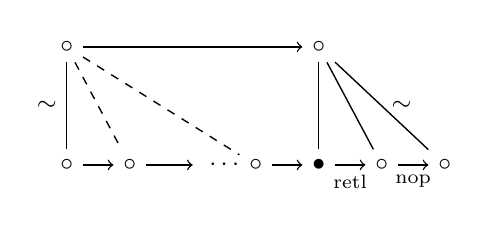
\begin{tikzpicture}[font=\small, line width=0.5pt]
    \node(S1) at (0, 1.5) {$\circ$};
    \node(S2) at (3.2, 1.5) {$\circ$};

    %%%%%%%%%%%%%%%%%%%%%%%%%%%%%%%%%%%%%%%%%%%%%%
    \node(T1) at (0, 0) {$\circ$};
    \node(T2) at (0.8, 0) {$\circ$};
    \node(T3) at (2.4, 0) {$\circ$};
    \node(T4) at (3.2, 0) {$\bullet$};
    \node(T5) at (4, 0) {$\circ$};
    \node(T6) at (4.8, 0) {$\circ$};

    %%%%%%%%%%%%%%%%%%%%%%%%%%%%%%%%%%%%%%%%%%%%%%
    \draw[-] (S1) to node[left]{$\sim$} (T1);
    \draw[-, dashed] (S1) to (T2);
    \draw[-, dashed] (S1) to (T3);
    \draw[-] (S2) to (T4);
    \draw[-] (S2) to (T5);
    \draw[-] (S2) to node[right]{$\sim$} (T6);

    \draw[->] (S1) to node[above]{\scriptsize $\primsw{}$} (S2);

    \draw[->] (T1) to (T2);
    \draw[->] (T2) to (1.6, 0);
    \node(dots) at (2, 0) {$\cdots$};
    \draw[->] (T3) to (T4);
    \draw[->] (T4) to node[below]{\scriptsize retl} (T5);
    \draw[->] (T5) to node[below]{\scriptsize nop} (T6);

    % \node(hexec) at (3.2, -1) 
    %     {\scriptsize
    %     $\begin{array}{l}
    %         \text{apply } \myrule{ABSCSQ} \\
    %         \text{rule}
    %     \end{array}$};
\end{tikzpicture}